\chapter{臺南大學AI機器人場域驗證影片和艾倫圖靈的故事-模仿遊戲電影}

使用以下文本內容分別使用TAIDE, Zephyr, Llama 3模型產生知識圖。
\begin{longtblr}[
    caption = {臺南大學AI機器人場域驗證影片和艾倫圖靈的故事文本內容及知識圖},
]{
    colspec = {|Q[c]|Q[c]|},
    rowspec = {|Q[m]|Q[m]|},
    hlines,vlines,
    % width = 0.7\linewidth
}
% 文本
\begin{minipage}{0.4\textwidth}
    \raggedright
    \vspace{5pt}
    \small 
    National University of Tainan has developed a robot to help students learn Taiwanese.\\
    The robot uses AI to assist students in practicing speaking Taiwanese, creates learning notes, and generates images to support learning.
    \vspace{5pt}
\end{minipage} &  
\begin{minipage}{0.4\textwidth}
    \raggedright
    \vspace{5pt}
    \small 
    Alan Turing\\
    Sexual Orientation Persecution\\
    Codebreaking\\
    Computer Science
    \vspace{5pt}
\end{minipage} \\
% 知識圖
\begin{minipage}[t][5cm][b]{0.3\textwidth}
            \centering
            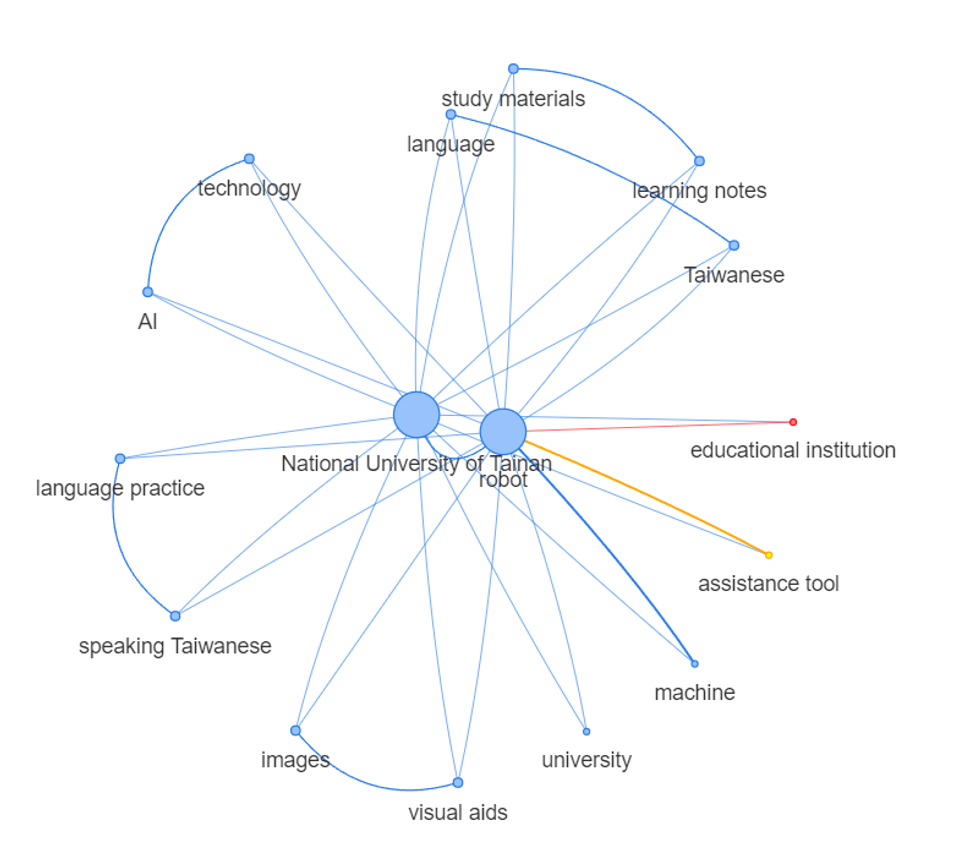
\includegraphics[width=\textwidth]{images/w2/w2_taide_1.png}\\
            \setcounter{figure}{0} % 将图像计数器重置为 0
            \captionsetup{font=scriptsize}
            \captionof{figure}{機器人場域驗證-TAIDE}
\end{minipage}  &  
\begin{minipage}[t][5cm][b]{0.3\textwidth}
            \centering
            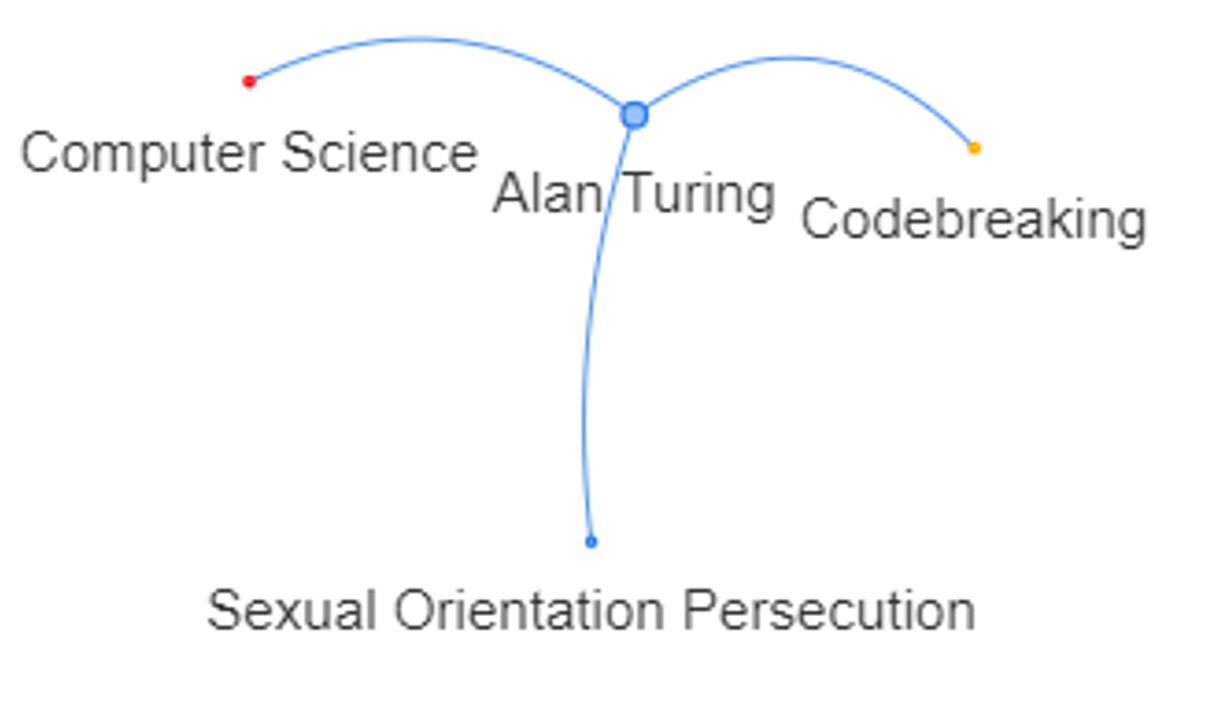
\includegraphics[width=\textwidth]{images/w2/w2_taide_2.png}\\
            \setcounter{figure}{1} 
            \captionsetup{font=scriptsize}
            \captionof{figure}{模仿遊戲-TAIDE}
        \end{minipage} \\
% 評分
\begin{minipage}[t]{0.4\textwidth}
            \centering
            \small \textbf{評分(1/10):9} \\
            \raggedright
            \small 原因: \par 1.有把重點台南大學使用機器人輔助教學和許多資訊連接在一起
            \vspace{5pt}
\end{minipage}  &  
\begin{minipage}[t]{0.4\textwidth}
            \centering
            \small \textbf{評分(1/10):4} \\
            \raggedright
            \small 原因: \par 1.資訊量少\par2.節點間關聯性弱
\end{minipage} \\
% 知識圖
\begin{minipage}[t][5cm][b]{0.3\textwidth}
            \centering
            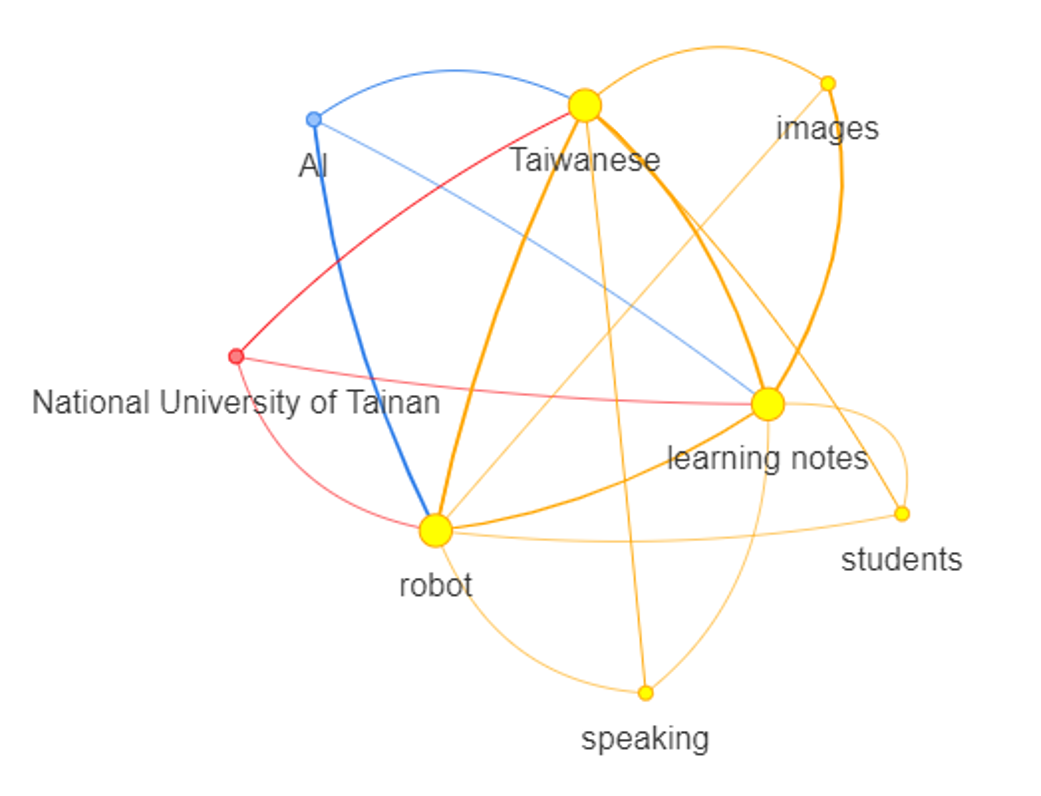
\includegraphics[width=\textwidth]{images/w2/w2_zephyr_1.png}\\
            \setcounter{figure}{2} 
            \captionsetup{font=scriptsize}
            \captionof{figure}{機器人場域驗證-Zephyr}
\end{minipage}  &  
\begin{minipage}[t][5cm][b]{0.3\textwidth}
            \centering
            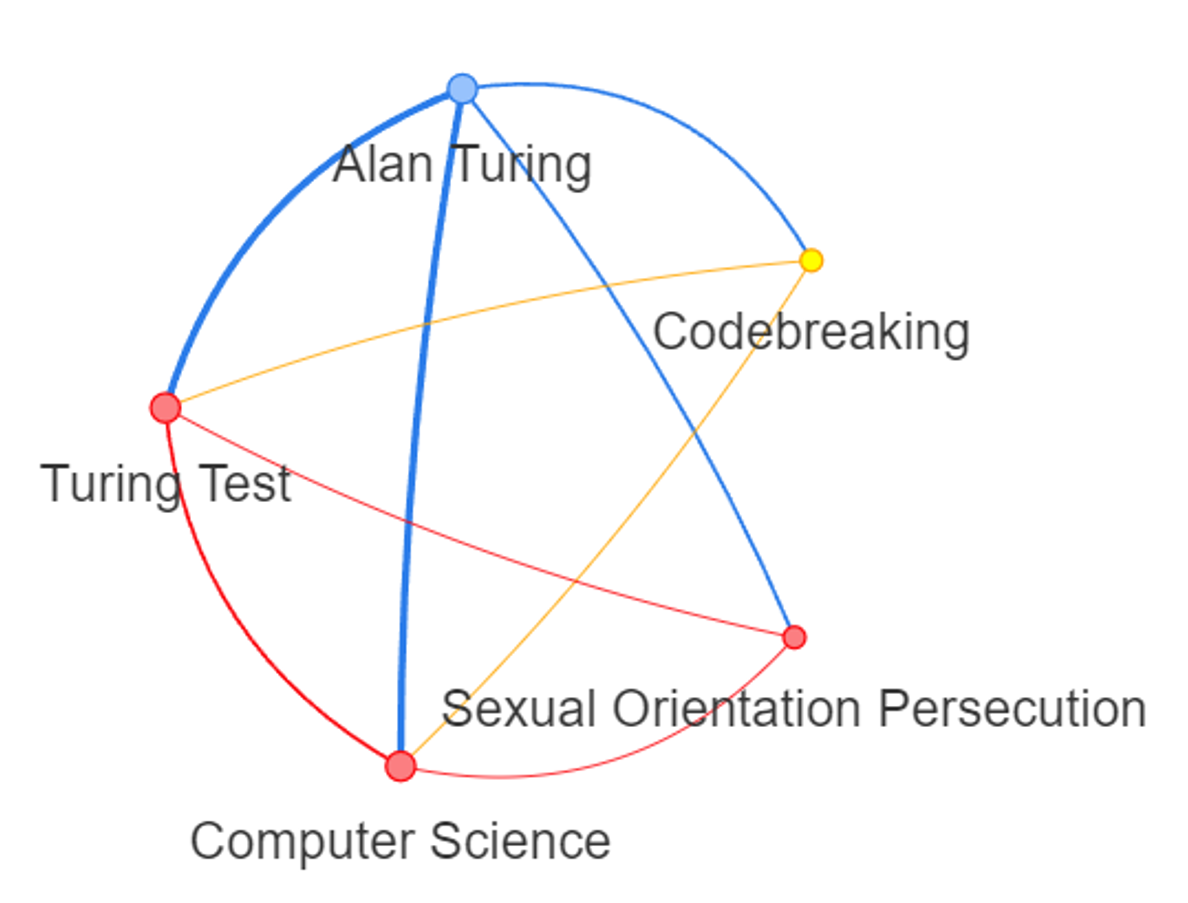
\includegraphics[width=\textwidth]{images/w2/w2_zephyr_2.png}\\
            \setcounter{figure}{3} 
            \captionsetup{font=scriptsize}
            \captionof{figure}{模仿遊戲-Zephyr}
        \end{minipage} \\
% 評分
\begin{minipage}[t]{0.4\textwidth}
            \centering
            \small \textbf{評分(1/10):8} \\
            \raggedright
            \small 原因: \par 1.資訊充足\par 2.連結性強但有點複雜不太容易看
            \vspace{5pt}
\end{minipage}  &  
\begin{minipage}[t]{0.4\textwidth}
            \centering
            \small \textbf{評分(1/10):7} \\
            \raggedright
            \small 原因: \par 1.彼此間的關聯性簡潔明瞭
\end{minipage} \\
% 知識圖
\begin{minipage}[t][5cm][b]{0.3\textwidth}
            \centering
            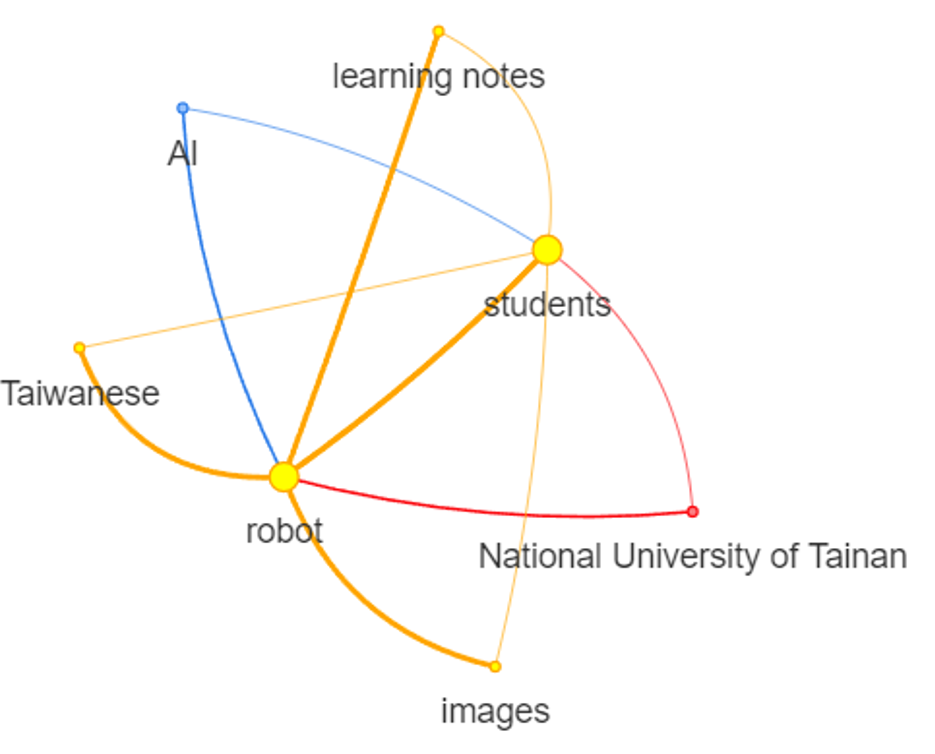
\includegraphics[width=\textwidth]{images/w2/w2_llama3_1.png}\\
            \setcounter{figure}{4}
            \captionsetup{font=scriptsize}
            \captionof{figure}{機器人場域驗證-Llama3}
\end{minipage}  &  
\begin{minipage}[t][5cm][b]{0.4\textwidth}
            \centering
            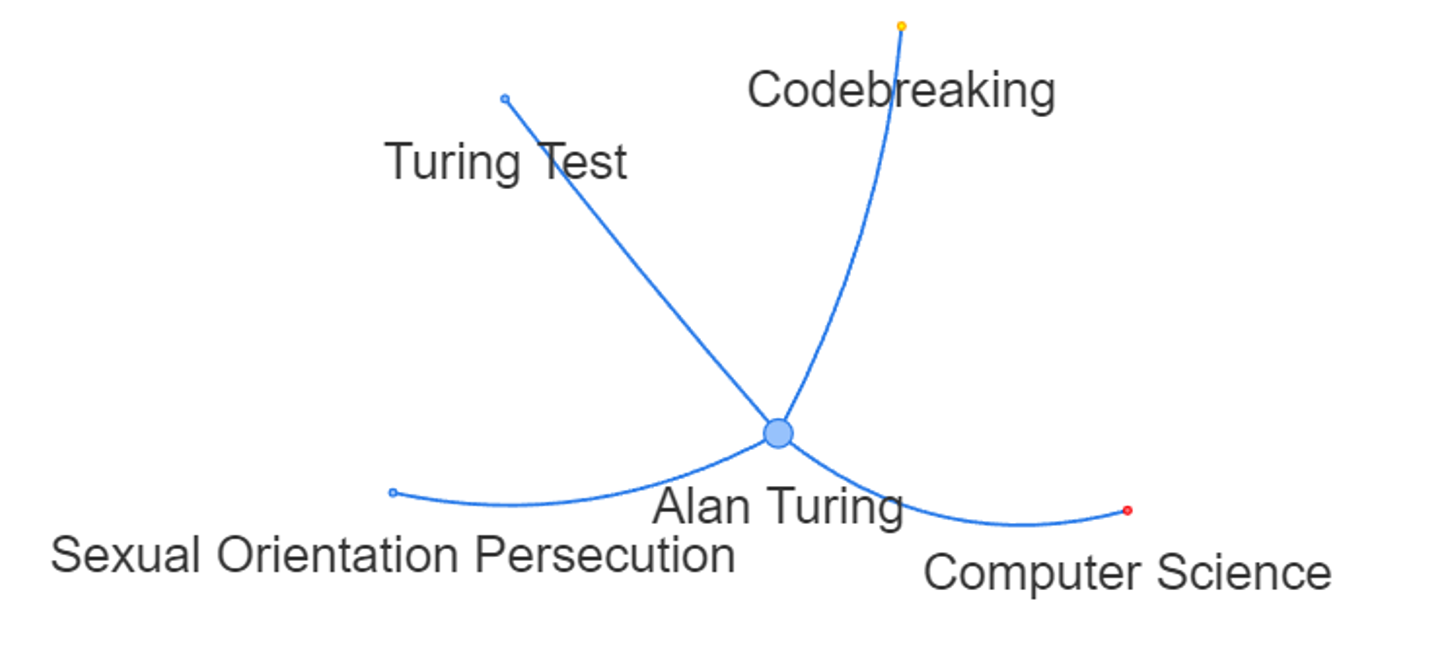
\includegraphics[width=\textwidth]{images/w2/w2_llama3_2.png}\\
            \setcounter{figure}{5} 
            \captionsetup{font=scriptsize}
            \captionof{figure}{模仿遊戲-Llama3}
        \end{minipage} \\
% 評分
\begin{minipage}[t]{0.4\textwidth}
            \centering
            \small \textbf{評分(1/10):7} \\
            \raggedright
            \small 原因: \par 1.彼此間的關聯性相對較少 \par
                             2.和Zephyr比起來少了speaking節點
            \vspace{5pt}
\end{minipage}  &  
\begin{minipage}[t]{0.4\textwidth}
            \centering
            \small \textbf{評分(1/10):5} \\
            \raggedright
            \small 原因: \par 1.資訊量少\par 2.節點間關聯性弱
\end{minipage} \\
\end{longtblr}
